\documentclass{standalone}
\usepackage{amsmath, amsfonts, amsthm}
\usepackage[dvipsnames]{xcolor}
\usepackage{siunitx}
\usepackage{graphicx}
\usepackage{tikz}
\usepackage{circuitikz}
\usetikzlibrary{patterns}
\usepackage{scalerel}
\usepackage{pict2e}
\usepackage{tkz-euclide}
\usetikzlibrary{calc}
\usetikzlibrary{arrows.meta}
\usetikzlibrary{shadows}
\usetikzlibrary{external}
\usetikzlibrary{decorations.pathmorphing}
\usetikzlibrary{shapes.geometric}
\usetikzlibrary{arrows,shapes.gates.logic.US,shapes.gates.logic.IEC,calc}
\usepackage{pgfplots}
\pgfplotsset{compat=newest}
\usepgfplotslibrary{statistics}
\usepgfplotslibrary{fillbetween}

\begin{document}
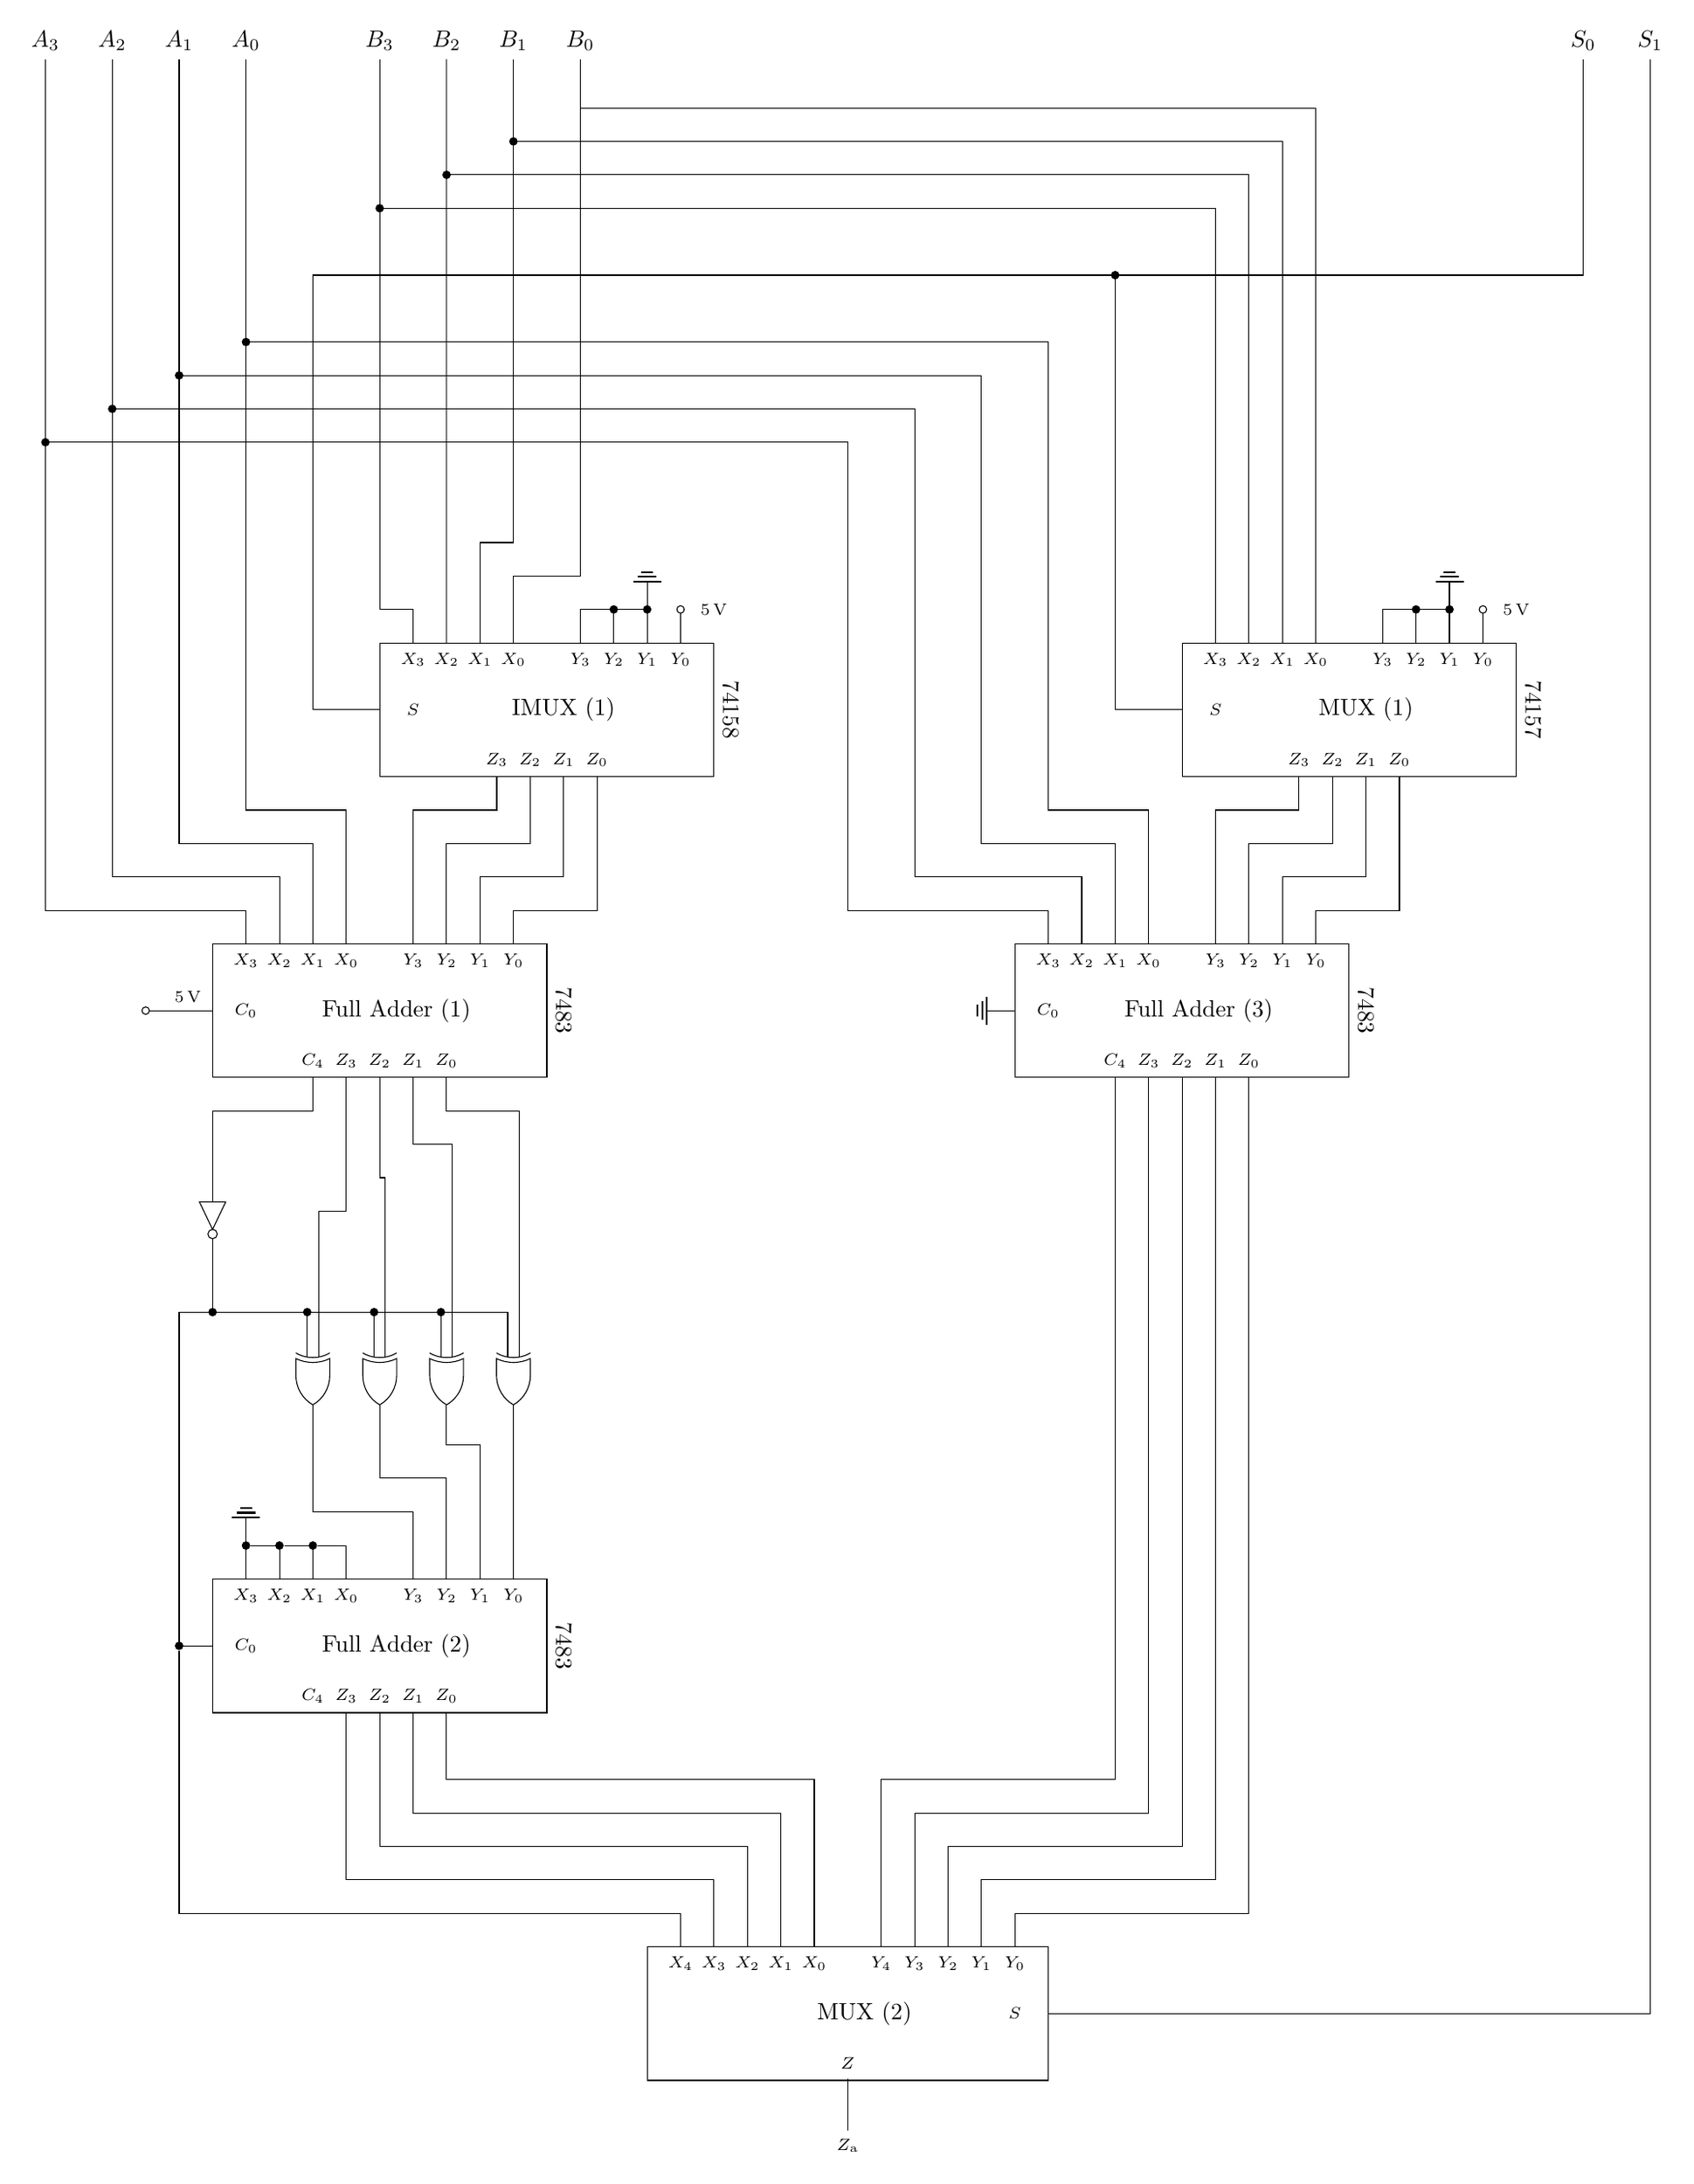
\begin{tikzpicture}
	%\draw [help lines, step=0.1, gray] (0,0) grid (10, -10);
	%\draw [help lines, blue] (0,0) grid (25, -40);

	\node (A3) at (0,0)      {$A_3$};
	\node (A2) [right of=A3] {$A_2$};
	\node (A1) [right of=A2] {$A_1$};
	\node (A0) [right of=A1] {$A_0$};

	\node (B3) [right of=A0, shift={(1, 0)}] {$B_3$};
	\node (B2) [right of=B3] {$B_2$};
	\node (B1) [right of=B2] {$B_1$};
	\node (B0) [right of=B1] {$B_0$};

	\node (S0) [right of=B0, shift={(14, 0)}] {$S_0$};
	\node (S1) [right of=S0] {$S_1$};

	% NotMux (1)

	\node (IMUX) [below of=B3, shift={(0, -8)}] { };
	\draw [black, thin] (IMUX) rectangle ++(5, -2);

	\node (IMUXX3) [font=\scriptsize, right of=IMUX, shift={(-.5, -.25)}] {$X_3$};
	\node (IMUXX2) [font=\scriptsize, right of=IMUXX3, shift={(-.5, 0)}] {$X_2$};
	\node (IMUXX1) [font=\scriptsize, right of=IMUXX2, shift={(-.5, 0)}] {$X_1$};
	\node (IMUXX0) [font=\scriptsize, right of=IMUXX1, shift={(-.5, 0)}] {$X_0$};

	\node (IMUXY3) [font=\scriptsize, right of=IMUXX0] {$Y_3$};
	\node (IMUXY2) [font=\scriptsize, right of=IMUXY3, shift={(-.5, 0)}] {$Y_2$};
	\node (IMUXY1) [font=\scriptsize, right of=IMUXY2, shift={(-.5, 0)}] {$Y_1$};
	\node (IMUXY0) [font=\scriptsize, right of=IMUXY1, shift={(-.5, 0)}] {$Y_0$};

	\node (IMUXS) [font=\scriptsize, below of=IMUXX3, shift={(0, .25)}] {$S$};

	\node (IMUXname) [rotate=-90, right of=IMUXY0, shift={(-.25, .75)}] {$74158$};
	\node (IMUXtag) [below of=IMUXX0, shift={(.75, .25)}] {IMUX (1)};

	\node (IMUXZ3) [font=\scriptsize, below of=IMUXX0, shift={(-.25, -.5)}] {$Z_3$};
	\node (IMUXZ2) [font=\scriptsize, right of=IMUXZ3, shift={(-.5, 0)}] {$Z_2$};
	\node (IMUXZ1) [font=\scriptsize, right of=IMUXZ2, shift={(-.5, 0)}] {$Z_1$};
	\node (IMUXZ0) [font=\scriptsize, right of=IMUXZ1, shift={(-.5, 0)}] {$Z_0$};

	\node (0s) [shift={(0, .75)}, ground, draw, rotate=180] at (IMUXY1) { };
	\node (1s) [ocirc, shift={(0.5, 0)}] at (0s) { };
	\node [font=\scriptsize, right of=1s, shift={(-0.5, 0)}] {$\qty{5}{V}$};

	\draw [shorten >=8] (S0)  -- ++(0, -3.5) -- ++(-19, 0) |- (IMUXS);

	\draw [shorten <=0.5] (IMUXX3) -- ++(0, .75) -| (B3);
	\draw [shorten <=0.5] (IMUXX2) --  (B2);
	\draw [shorten <=0.5] (IMUXX1) -- ++(0, 1.75) -| (B1);
	\draw [shorten <=0.5] (IMUXX0) -- ++(0, 1.25) -| (B0);

	\draw [shorten >=0.5] (0s)  node[circ] (0sn0) { } -| (IMUXY3);
	\draw [shorten >=0.5] (0s) -- (IMUXY1);
	\draw [shorten >=0.5] (0sn0) -- ++(-0.5, 0) node[circ] { } -| (IMUXY2);
	\draw [shorten >=0.5] (1s) -- (IMUXY0);

	% Full Adder (1)

	\node (Add1) [below of=IMUX, shift={(-2.5, -3.5)}] { };
	\draw [black, thin] (Add1) rectangle ++(5, -2);

	\node (Add1X3) [font=\scriptsize, right of=Add1, shift={(-.5, -.25)}] {$X_3$};
	\node (Add1X2) [font=\scriptsize, right of=Add1X3, shift={(-.5, 0)}] {$X_2$};
	\node (Add1X1) [font=\scriptsize, right of=Add1X2, shift={(-.5, 0)}] {$X_1$};
	\node (Add1X0) [font=\scriptsize, right of=Add1X1, shift={(-.5, 0)}] {$X_0$};

	\node (Add1Y3) [font=\scriptsize, right of=Add1X0] {$Y_3$};
	\node (Add1Y2) [font=\scriptsize, right of=Add1Y3, shift={(-.5, 0)}] {$Y_2$};
	\node (Add1Y1) [font=\scriptsize, right of=Add1Y2, shift={(-.5, 0)}] {$Y_1$};
	\node (Add1Y0) [font=\scriptsize, right of=Add1Y1, shift={(-.5, 0)}] {$Y_0$};

	\node (Add1C0) [font=\scriptsize, below of=Add1X3, shift={(0, .25)}] {$C_0$};

	\node (Add1name) [rotate=-90, right of=Add1Y0, shift={(-.25, .75)}] {$7483$};
	\node (Add1tag) [below of=Add1X0, shift={(.75, .25)}] {Full Adder (1)};

	\node (Add1Z3) [font=\scriptsize, below of=Add1X0, shift={(0, -.5)}] {$Z_3$};
	\node (Add1C4) [font=\scriptsize, left of=Add1Z3, shift={(.5, 0)}] {$C_4$};
	\node (Add1Z2) [font=\scriptsize, right of=Add1Z3, shift={(-.5, 0)}] {$Z_2$};
	\node (Add1Z1) [font=\scriptsize, right of=Add1Z2, shift={(-.5, 0)}] {$Z_1$};
	\node (Add1Z0) [font=\scriptsize, right of=Add1Z1, shift={(-.5, 0)}] {$Z_0$};

	\node [ocirc, left of=Add1, shift={(0, -1)}] (1C0) { };
	\draw [shorten >=6] (1C0.east) -- (Add1C0) node[midway, above, font=\scriptsize] {$\qty{5}{V}$};

	\draw [shorten <=0.5] (Add1X3) -- ++(0, .75) -| (A3);
	\draw [shorten <=0.5] (Add1X2) -- ++(0, 1.25) -| (A2);
	\draw [shorten <=0.5] (Add1X1) -- ++(0, 1.75) -| (A1);
	\draw [shorten <=0.5] (Add1X0) -- ++(0, 2.25) -| (A0);

	\draw [shorten >=0.5, shorten <=0.5] (IMUXZ3) -- ++(0, -.75) -| (Add1Y3);
	\draw [shorten >=0.5, shorten <=0.5] (IMUXZ2) -- ++(0, -1.25) -| (Add1Y2);
	\draw [shorten >=0.5, shorten <=0.5] (IMUXZ1) -- ++(0, -1.75) -| (Add1Y1);
	\draw [shorten >=0.5, shorten <=0.5] (IMUXZ0) -- ++(0, -2.25) -| (Add1Y0);

	\node [not gate US, draw, rotate=-90, below of=Add1, shift={(4, 1)}] ('C4) { };
	\node [xor gate US, draw, rotate=-90, logic gate inputs=nn, below of=Add1C4, shift={(4.75, 1)}] (Xor3) { };
	\node [xor gate US, draw, rotate=-90, logic gate inputs=nn, above of=Xor3] (Xor2) { };
	\node [xor gate US, draw, rotate=-90, logic gate inputs=nn, above of=Xor2] (Xor1) { };
	\node [xor gate US, draw, rotate=-90, logic gate inputs=nn, above of=Xor1] (Xor0) { };

	\draw [shorten <=0.5] (Add1C4) -- ++(0, -.75) -| ('C4.input);

	\draw ('C4.output) -- ++(0, -1.09) node[circ] (sign) {} -| node[circ](sign3) { } (Xor3.input 2);
	\draw (sign3) -| node[circ](sign2) { } (Xor2.input 2);
	\draw (sign2) -| node[circ](sign1) { } (Xor1.input 2);
	\draw (sign1) -| (Xor0.input 2);

	\draw [shorten <=.5] (Add1Z3) -- ++(0, -2.25) -| (Xor3.input 1);
	\draw [shorten <=.5] (Add1Z2) -- ++(0, -1.75) -| (Xor2.input 1);
	\draw [shorten <=.5] (Add1Z1) -- ++(0, -1.25) -| (Xor1.input 1);
	\draw [shorten <=.5] (Add1Z0) -- ++(0, -.75) -| (Xor0.input 1);

	% Full Adder (2)

	\node (Add2) [below of='C4, shift={(0, -4.5)}] { };
	\draw [black, thin] (Add2) rectangle ++(5, -2);

	\node (Add2X3) [font=\scriptsize, right of=Add2, shift={(-.5, -.25)}] {$X_3$};
	\node (Add2X2) [font=\scriptsize, right of=Add2X3, shift={(-.5, 0)}] {$X_2$};
	\node (Add2X1) [font=\scriptsize, right of=Add2X2, shift={(-.5, 0)}] {$X_1$};
	\node (Add2X0) [font=\scriptsize, right of=Add2X1, shift={(-.5, 0)}] {$X_0$};

	\node (Add2Y3) [font=\scriptsize, right of=Add2X0] {$Y_3$};
	\node (Add2Y2) [font=\scriptsize, right of=Add2Y3, shift={(-.5, 0)}] {$Y_2$};
	\node (Add2Y1) [font=\scriptsize, right of=Add2Y2, shift={(-.5, 0)}] {$Y_1$};
	\node (Add2Y0) [font=\scriptsize, right of=Add2Y1, shift={(-.5, 0)}] {$Y_0$};

	\node (Add2C0) [font=\scriptsize, below of=Add2X3, shift={(0, .25)}] {$C_0$};

	\node (Add2name) [rotate=-90, right of=Add2Y0, shift={(-.25, .75)}] {$7483$};
	\node (Add2tag) [below of=Add2X0, shift={(.75, .25)}] {Full Adder (2)};

	\node (Add2Z3) [font=\scriptsize, below of=Add2X0, shift={(0, -.5)}] {$Z_3$};
	\node (Add2C4) [font=\scriptsize, left of=Add2Z3, shift={(.5, 0)}] {$C_4$};
	\node (Add2Z2) [font=\scriptsize, right of=Add2Z3, shift={(-.5, 0)}] {$Z_2$};
	\node (Add2Z1) [font=\scriptsize, right of=Add2Z2, shift={(-.5, 0)}] {$Z_1$};
	\node (Add2Z0) [font=\scriptsize, right of=Add2Z1, shift={(-.5, 0)}] {$Z_0$};

	\node (0c) [ground, draw, rotate=-180, below of=Add2X3, shift={(0, +.25)}] { };
	\draw [shorten <=0.5, shorten >=.5] (0c) node[circ](0c3) { } -- (Add2X3);
	\draw [shorten <=0.5, shorten >=.5] (0c3) -| node[circ](0c2) { } (Add2X2);
	\draw [shorten <=0.5, shorten >=.5] (0c2) -| node[circ](0c1) { } (Add2X1);
	\draw [shorten <=0.5, shorten >=.5] (0c1) -| (Add2X0);

	\draw [shorten >=6] (sign) -- ++(-0.5, 0) |- node[circ](cAdd1C0) { } (Add2C0);

	\draw [shorten >=.5] (Xor3.output) -- ++(0, -1.59) -| (Add2Y3);
	\draw [shorten >=.5] (Xor2.output) -- ++(0, -1.09) -| (Add2Y2);
	\draw [shorten >=.5] (Xor1.output) -- ++(0, -.59) -| (Add2Y1);
	\draw [shorten >=.5] (Xor0.output) -- (Add2Y0);

	% MUX (1)

	\node (MUX) [right of=IMUX, shift={(11, 0)}] { };
	\draw [black, thin] (MUX) rectangle ++(5, -2);

	\node (MUXX3) [font=\scriptsize, right of=MUX, shift={(-.5, -.25)}] {$X_3$};
	\node (MUXX2) [font=\scriptsize, right of=MUXX3, shift={(-.5, 0)}] {$X_2$};
	\node (MUXX1) [font=\scriptsize, right of=MUXX2, shift={(-.5, 0)}] {$X_1$};
	\node (MUXX0) [font=\scriptsize, right of=MUXX1, shift={(-.5, 0)}] {$X_0$};

	\node (MUXY3) [font=\scriptsize, right of=MUXX0] {$Y_3$};
	\node (MUXY2) [font=\scriptsize, right of=MUXY3, shift={(-.5, 0)}] {$Y_2$};
	\node (MUXY1) [font=\scriptsize, right of=MUXY2, shift={(-.5, 0)}] {$Y_1$};
	\node (MUXY0) [font=\scriptsize, right of=MUXY1, shift={(-.5, 0)}] {$Y_0$};

	\node (MUXS) [font=\scriptsize, below of=MUXX3, shift={(0, .25)}] {$S$};

	\node (MUXname) [rotate=-90, right of=MUXY0, shift={(-.25, .75)}] {$74157$};
	\node (MUXtag) [below of=MUXX0, shift={(.75, .25)}] {MUX (1)};

	\node (MUXZ3) [font=\scriptsize, below of=MUXX0, shift={(-.25, -.5)}] {$Z_3$};
	\node (MUXZ2) [font=\scriptsize, right of=MUXZ3, shift={(-.5, 0)}] {$Z_2$};
	\node (MUXZ1) [font=\scriptsize, right of=MUXZ2, shift={(-.5, 0)}] {$Z_1$};
	\node (MUXZ0) [font=\scriptsize, right of=MUXZ1, shift={(-.5, 0)}] {$Z_0$};

	\node (0a) [shift={(0, .75)}, ground, draw, rotate=180] at (MUXY1) { };
	\node (1a) [ocirc, shift={(0.5, 0)}] at (0a) { };
	\node [font=\scriptsize, right of=1a, shift={(-0.5, 0)}] {$\qty{5}{V}$};

	\draw [shorten >=0.5] (0a) node[circ] (0an0) { } -| (MUXY3);
	\draw [shorten >=0.5] (0a) -- (MUXY1);
	\draw [shorten >=0.5] (0an0) -- ++(-0.5, 0) node[circ] { } -| (MUXY2);
	\draw [shorten >=0.5] (1a) -- (MUXY0);

	\draw [shorten >=.5] (B0) ++(0, -1)  -| (MUXX0);
	\draw [shorten >=.5] (B1) ++(0, -1.5) node[circ] { } -| (MUXX1);
	\draw [shorten >=.5] (B2) ++(0, -2) node[circ] { } -| (MUXX2);
	\draw [shorten >=.5] (B3) ++(0, -2.5) node[circ] { } -| (MUXX3);

	\draw [shorten <=8] (MUXS) -- ++(-1.5, 0) -- ++(0, 6.5) node[circ] { };

	% Full Adder (3)

	\node (Add3) [below of=MUX, shift={(-2.5, -3.5)}] { };
	\draw [black, thin] (Add3) rectangle ++(5, -2);

	\node (Add3X3) [font=\scriptsize, right of=Add3, shift={(-.5, -.25)}] {$X_3$};
	\node (Add3X2) [font=\scriptsize, right of=Add3X3, shift={(-.5, 0)}] {$X_2$};
	\node (Add3X1) [font=\scriptsize, right of=Add3X2, shift={(-.5, 0)}] {$X_1$};
	\node (Add3X0) [font=\scriptsize, right of=Add3X1, shift={(-.5, 0)}] {$X_0$};

	\node (Add3Y3) [font=\scriptsize, right of=Add3X0] {$Y_3$};
	\node (Add3Y2) [font=\scriptsize, right of=Add3Y3, shift={(-.5, 0)}] {$Y_2$};
	\node (Add3Y1) [font=\scriptsize, right of=Add3Y2, shift={(-.5, 0)}] {$Y_1$};
	\node (Add3Y0) [font=\scriptsize, right of=Add3Y1, shift={(-.5, 0)}] {$Y_0$};

	\node (Add3C0) [font=\scriptsize, below of=Add3X3, shift={(0, .25)}] {$C_0$};

	\node (Add3name) [rotate=-90, right of=Add3Y0, shift={(-.25, .75)}] {$7483$};
	\node (Add3tag) [below of=Add3X0, shift={(.75, .25)}] {Full Adder (3)};

	\node (Add3Z3) [font=\scriptsize, below of=Add3X0, shift={(0, -.5)}] {$Z_3$};
	\node (Add3C4) [font=\scriptsize, left  of=Add3Z3, shift={(.5, 0)}] {$C_4$};
	\node (Add3Z2) [font=\scriptsize, right of=Add3Z3, shift={(-.5, 0)}] {$Z_2$};
	\node (Add3Z1) [font=\scriptsize, right of=Add3Z2, shift={(-.5, 0)}] {$Z_1$};
	\node (Add3Z0) [font=\scriptsize, right of=Add3Z1, shift={(-.5, 0)}] {$Z_0$};

	\node [ground, draw, below of=Add3, rotate=-90] { };

	\draw [shorten <=0.5] (Add3X3) -- ++(0, .75) -- ++(-3, 0) -- ++(0, 7) -| node[circ] { } (A3);
	\draw [shorten <=0.5] (Add3X2) -- ++(0, 1.25) -- ++(-2.5, 0) -- ++(0, 7) -| node[circ] { } (A2);
	\draw [shorten <=0.5] (Add3X1) -- ++(0, 1.75) -- ++(-2, 0) -- ++(0, 7) -| node[circ] { } (A1);
	\draw [shorten <=0.5] (Add3X0) -- ++(0, 2.25) -- ++(-1.5, 0) -- ++(0, 7) -| node[circ] { } (A0);

	\draw [shorten >=0.5, shorten <=0.5] (MUXZ3) -- ++(0, -.75) -| (Add3Y3);
	\draw [shorten >=0.5, shorten <=0.5] (MUXZ2) -- ++(0, -1.25) -| (Add3Y2);
	\draw [shorten >=0.5, shorten <=0.5] (MUXZ1) -- ++(0, -1.75) -| (Add3Y1);
	\draw [shorten >=0.5, shorten <=0.5] (MUXZ0) -- ++(0, -2.25) -| (Add3Y0);

	% MUX (2)

	\node (MUX2) [below of=Add2, shift={(6.5, -4.5)}] { };
	\draw [black, thin] (MUX2) rectangle ++(6, -2);

	\node (MUX2X4) [font=\scriptsize, right of=MUX2, shift={(-.5, -.25)}] {$X_4$};
	\node (MUX2X3) [font=\scriptsize, right of=MUX2X4, shift={(-.5, 0)}] {$X_3$};
	\node (MUX2X2) [font=\scriptsize, right of=MUX2X3, shift={(-.5, 0)}] {$X_2$};
	\node (MUX2X1) [font=\scriptsize, right of=MUX2X2, shift={(-.5, 0)}] {$X_1$};
	\node (MUX2X0) [font=\scriptsize, right of=MUX2X1, shift={(-.5, 0)}] {$X_0$};

	\node (MUX2Y4) [font=\scriptsize, right of=MUX2X0] {$Y_4$};
	\node (MUX2Y3) [font=\scriptsize, right of=MUX2Y4, shift={(-.5, 0)}] {$Y_3$};
	\node (MUX2Y2) [font=\scriptsize, right of=MUX2Y3, shift={(-.5, 0)}] {$Y_2$};
	\node (MUX2Y1) [font=\scriptsize, right of=MUX2Y2, shift={(-.5, 0)}] {$Y_1$};
	\node (MUX2Y0) [font=\scriptsize, right of=MUX2Y1, shift={(-.5, 0)}] {$Y_0$};

	\node (MUX2S) [font=\scriptsize, below of=MUX2Y0, shift={(0, .25)}] {$S$};

	\node (MUX2tag) [below of=MUX2X0, shift={(.75, .25)}] {MUX (2)};

	\node (MUX2Z) [font=\scriptsize, below of=MUX2X0, shift={(.5, -.5)}] {$Z$};

	\draw [shorten <=0.5, shorten >=0.5] (cAdd1C0) -- ++(0, -4)   - | (MUX2X4);
	\draw [shorten <=0.5, shorten >=0.5] (Add2Z3) -- ++(0, -2.75) - | (MUX2X3);
	\draw [shorten <=0.5, shorten >=0.5] (Add2Z2) -- ++(0, -2.25) - | (MUX2X2);
	\draw [shorten <=0.5, shorten >=0.5] (Add2Z1) -- ++(0, -1.75) - | (MUX2X1);
	\draw [shorten <=0.5, shorten >=0.5] (Add2Z0) -- ++(0, -1.25) - | (MUX2X0);

	\draw [shorten <=0.5, shorten >=0.5] (MUX2Y4) -- ++(0, 2.75) - | (Add3C4);
	\draw [shorten <=0.5, shorten >=0.5] (MUX2Y3) -- ++(0, 2.25) - | (Add3Z3);
	\draw [shorten <=0.5, shorten >=0.5] (MUX2Y2) -- ++(0, 1.75) - | (Add3Z2);
	\draw [shorten <=0.5, shorten >=0.5] (MUX2Y1) -- ++(0, 1.25) - | (Add3Z1);
	\draw [shorten <=0.5, shorten >=0.5] (MUX2Y0) -- ++(0, .75)  - | (Add3Z0);

	\draw [shorten >=8] (S1) |- (MUX2S);

	\draw [shorten <=0.5] (MUX2Z) -- ++(0, -1) node[font=\scriptsize, below] {$Z_{\text{a}}$};

\end{tikzpicture}
\end{document}
